%\vspace*{\subsecspace}
\section{Design: Scheduling GPU Functions}
\vspace*{\subsecspace}
\label{sec:design}

The main new contribution and component of our hybrid serverless computing platform is the scheduler for GPU functions, which we describe in this section. 
The different hardware and workload model of GPUs requires a different approach to scheduling as compared to conventional CPU function scheduling. 
To tackle these challenges, we first show that fair queuing as used in I/O scheduling can be a useful framework for GPU scheduling (Section~\ref{sec:d:mqfq}), then describe the GPU-specific scheduling (Section~\ref{sec:mq}) and memory management optimizations (Section~\ref{sec:design-cont-shim}). 

\begin{figure}
  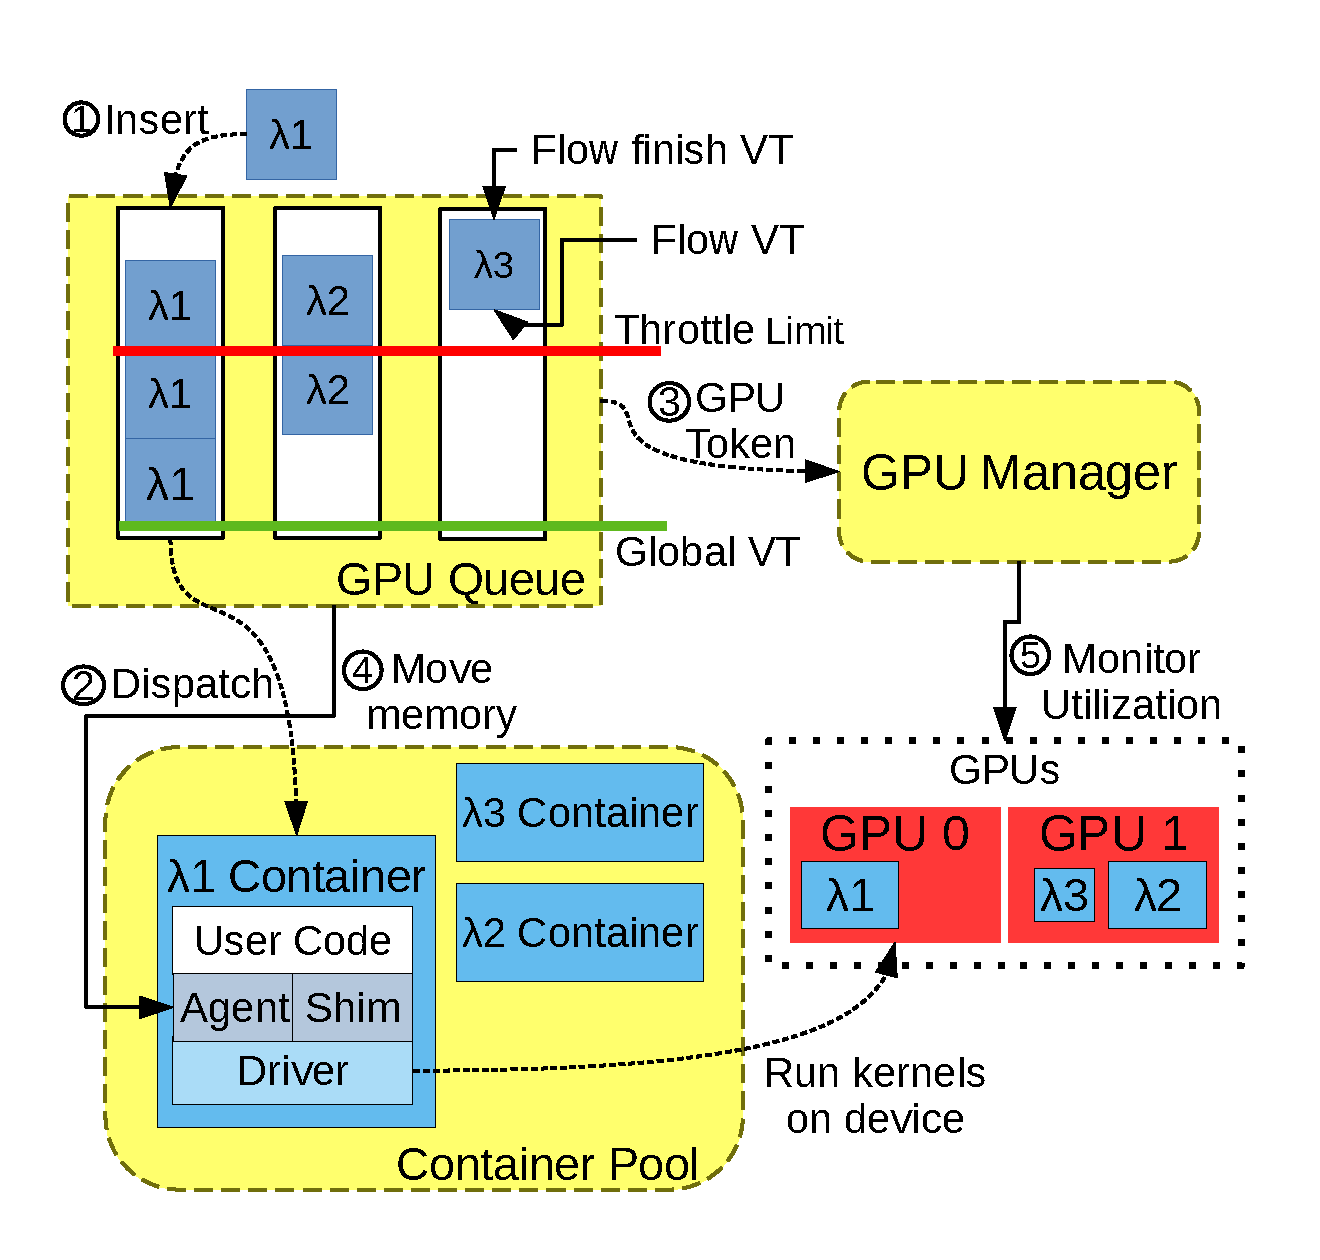
\includegraphics[width=0.5\textwidth]{../figs/queue-sys-2-simple.pdf}
  \vspace*{-0.8cm}
  \caption{Scheduling GPU functions as flows with Multi-Queue Fair Queuing. Invocations are dispatched based on the virtual time. The container pool helps with warm starts.}
  \vspace{-0.25cm}
  \label{fig:sys-diag}
  % \vspace{-0.6cm}
\end{figure}


\subsection{Key Insight: GPUs as Multi-Queue I/O Devices}
\label{sec:d:mqfq}

We claim that the tradeoffs and challenges of guaranteeing fairness and high throughput for serverless GPU workloads are similar to modern I/O scheduling.
Specifically, we can view GPUs as multi-queue I/O devices, and use fair scheduling algorithms like MQFQ~\cite{hedayati2019multi} to provide a rigorous and well-tested conceptual framework.
From a workload perspective, the I/O heterogeneity and fairness of different applications is similar to FaaS functions' heterogeneity.
Similarly, modern disks have multiple internal dispatch queues, which also maps to the temporal and spatial multiplexing offered by GPUs.
Successive invocations see lower latency from temporal and even spatial locality, a fact requiring significant attention when maximizing throughput.

Our scheduler maintains multiple dispatch queues, each queue corresponding to an individual function.
These queues (also called \emph{flows}) hold invocation requests which are analogous to disk read/write requests.
Multiple invocations dispatched from a single flow preserve temporal locality and benefit from warm starts.
The GPU, just like modern NVMe disks, also supports parallel dispatches, and we keep a subset of flows in the \quotes{active} state.
Flows without en-queued invocations are \quotes{inactive}.
Fair queuing uses the notion of virtual time (\VT) to capture the amount of service rendered to flows (normalized by priority weight).
The flow's \VT~grows by a fixed increment after an item is removed and dispatched for execution.
Flows are selected for dispatch based on their \VT's, and fairness arises from a bound on the maximum difference of flows \VT's.

Our insight is that the above classic fair queuing framework can be extended to meet the challenges of serverless GPU scheduling.
Locality is maintained by dispatching successive requests from an active flow, by borrowing ideas from anticipatory scheduling and using MQFQ's concurrent dispatch, which increases throughput but still maintains fairness (albeit with a larger inter-flow \VT~bound compared to classic fair queuing with a single active flow).
Each flow can be handled by a separate thread which can dispatch requests concurrently, taking advantage of device-level parallelism.
The amount of device parallelism is configured and controlled via tokens with the \D~parameter (Table~\ref{tab:mq-symbols}). 
To prevent popular functions from monopolizing the GPU, flows are \emph{throttled} if their \VT~exceeds the global \VT~(\GlobVT) (which is the minimum of all flows' \VT) by a certain threshold (\T).
\emph{Fair queuing provides the necessary parameters for principled and tunable batching in an online manner, for highly dynamic and heterogeneous FaaS workloads.}

\begin{table}
  \caption{Key symbols and parameters for \QName.}
  \label{tab:mq-symbols}
  \vspace{\captionspace}
  \begin{tabular}{c|p{6.2cm}}
    \hline
    Symbol & Description \\
    \hline
    \VT & Virtual Time, device wall clock service time accrued by a flow \\
    \GlobVT & Minimum \VT~across all active flows \\
    \T & Amount any flow's \VT~can exceed \GlobVT~before being throttled \\
    \D & Device concurrent invocations, can be fixed or dynamic with an upper-bound \\
    % \FinVT & A Flows \quotes{Finish}~\VT, the flow's \VT~plus its length by average execution time \\
    TTL & Time-to-live for an empty flow to become inactive \\
    % Service Average & Amount by which a flow's \VT~is increased after dispatch \\
  \end{tabular}
  \vspace{-0.4cm}
\end{table}

\subsection{MQFQ-Sticky: Locality-enhanced Fair Queuing}
\label{sec:mq}

% Want to enhance the locality of MQFQ.

The above MQFQ scheduling framework was designed for I/O.
However, GPU functions have different compute and memory footprints, execution runtimes, and cold vs. warm execution times; all of which diverge from disk assumptions. 
The GPU device model is also different: the device parallelism is lower (SSDs support hundreds of active threads), and execution performance is highly sensitive to utilization and interference. 
We therefore modify the original MQFQ design to account for these differences, to get the maximum performance out of our accelerators. 

% Tasks sent to sold-state disk I/O use equal amounts of device time and resources.
% Their GPU function counterparts can vary widely in both of these metrics, including between invocations of the same function.
% Disks can also handle over 100 parallel requests, and GPUs see execution overhead with single-digit concurrency that also is dependent on compute and memory usage.

Unlike disk requests with uniform block sizes, function execution times can vary significantly.
% This is a NOVELTY of ours, not in MQFQ. Also VT is not updated on insertion, that statement is wrong. You're thinking of the per-invocation VT / a flows Finish VT being incremented
% A new invocation is inserted into its function's flow, and the flow's \VT~is incremented based on the function's expected execution times. 
We account for this by tracking the historical average execution time $\tau_k$ of each function $k$, and when an item is dispatched, its flow's \VT~is instead incremented by $\tau_k/w_k$, where $w_k$ is the priority weight of the function.
Thus shorter functions are allowed more \emph{invocations} than their long counterparts, but both get equivalent wall time on the GPU.
% WRONG. Always updates to the GLOBAL MINIMUM across all flows. Updating like this causes serious divergence in global VT
% When an invocation is dispatched, the global \VT~is updated to the flow's \VT~as long as the \GlobVT~monotonically increases (i.e., $\GlobVT~= max(\GlobVT, flow.\VT)$). 
After an invocation is dispatched, \GlobVT~is updated if necessary to a potentially new global minima across flow VTs.
%(i.e. $\GlobVT~=~min(\forall flow.\VT~\in~Flows)$).

Since GPU memory is limited, we use the flow states for \textbf{proactive memory management.}
Flows that become active have their data moved onto the device in anticipation of use (if space is available). 
When a container is about to execute, we proactively move all its data to the GPU. 
Conversely, throttled and inactive flows have their data moved off-device, because we don't expect them to run in the near future. 
% Reclaiming device memory allows us to warm an active flow's data, data movement details are described in Section~\ref{sec:design-cont-shim}. 
More details about the data monitoring and movement are described in Section~\ref{sec:design-cont-shim}. 
Further modifications of ours pertain to how functions are drained and added to the queues, and are described below. 

\mhead{Anticipatory Scheduling}
Function performance is impacted by the availability of a warm container, and data in GPU memory.  
We introduce anticipatory scheduling to MQFQ to maximize the use of both. 
Anticipatory scheduling for disks~\cite{iyer2001anticipatory} boosts locality by keeping request streams \quotes{active} even if they are empty, in anticipation of future requests, which is especially beneficial for interactive applications.  
If a flow is empty (i.e., it has no pending invocations), then instead of immediately marking it inactive, we provide a grace period.
Without this grace period, because of the proactive memory management described above, functions would see their warm containers immediately removed from GPU memory.
%
Instead, we keep empty flows active for a configurable TTL (time to live), based on the function's inter-arrival-times.
Specifically, we set the flow TTL to $\alpha \times \text{IAT}$, where $\alpha$ is a tunable parameter. 
This policy is guided by the observation that reuse-distance is long-tailed~\cite{faascache-asplos21}, so a single global TTL is not ideal for both popular and rare functions. 

\mhead{Flow Over-run}
Our second technique for improving warm starts is to allow the flows to dispatch invocations in small \quotes{mini-batches}.
An active flow's start time is allowed to be \T~units ahead of \GlobVT.
\T~is the second main configurable parameter: larger values will result in larger batches and more locality, but less fairness, since functions will have to wait longer before their batches are dispatched.
If $flow.\VT + \T \ge \GlobVT$, then the flow is \emph{throttled}.
It may return to the \emph{active} state only after other flows get to run and the \GlobVT~increases. 


\mhead{Device Concurrency and Feedback}
% A device's concurrency limit \D~is not pre-determined as in the disk case.
% We must 
Because each function uses different amounts of compute and memory during execution, a fixed level of device parallelism (\D) like in disk scheduling may be sub-optimal.
We therefore track memory usage of running containers and GPU utilization to adjust \D~dynamically, to minimize contention and execution overhead.
This utilization-based feedback permits different scheduling rates based on the dynamic workload characteristics.
We take two input parameters: the device utilization threshold (such as 90\%), and the maximum parallelism level (irrespective of utilization).
A coarse-grained controller loop runs every 200 ms to check the real-time utilization and changes the \D~level dynamically to ensure the utilization is under the threshold.
Higher thresholds increase utilization and reduce queuing, but risk higher performance interference. 
% These methods are described in detail in Sections~\ref{sec:gpu-man} and~\ref{sec:design-cont-shim}.
More details of memory usage and GPU monitoring are described in Section~\ref{sec:design-cont-shim} and Section~\ref{sec:gpu-man} respectively. 

\mhead{Dispatch Concurrency}
In classic MQFQ, flows can concurrently dispatch their requests (as long as they are within the \T~threshold).
From a FaaS control plane perspective which needs to track invocation status carefully, we prefer a \emph{single} dispatch thread which picks the eligible candidate flow queue (such that $flow.\VT < \GlobVT + \T$).
Thus, the dispatch is not concurrent, which results in the most fair outcome via selecting flow with the lowest \VT~(i.e., earliest arrival).
However, this reduces locality and batching opportunities, resulting in poor function performance.

To remedy this, we pick the next flow from the set of candidate flows by sorting on both recency and locality, as shown in line~\ref{lst:line:filter} of Algorithm~\ref{algo:dispatch}.
Our heuristic prefers longer queues which provide more batching opportunities and reduces their larger backlog.
Ties are broken in favor of the flow with the least number of currently executing invocations (Line~\ref{lst:line:in_flight}).
This encourages multiple flows to progress and reduces the chance of a cold start caused by concurrent execution of the same function.
% In both cases we are draining the most backed up queues and enabling flow stickiness.
Flow stickiness from this heuristic provides sufficient temporal locality between active flows to maximize throughput.
This completes the description of the key attributes of our MQFQ-Sticky algorithm.
We note that it maintains the fairness properties, since we are basically emulating dispatch concurrency, but prioritizing longer flows within the eligible flow window.
That is, we still retain the MQFQ fairness property, which states that the service received ($S$) by two active flows during a span of wall-clock time $(t_1, t_2)$ is bounded by:
\vspace{-0.1cm}
\begin{equation}
  \label{eq:fairness}
 \left|\dfrac{S_i}{w_i} - \dfrac{S_j}{w_j} \right| \leq (D-1) \left(2T + \dfrac{\tau_i}{w_i} -\dfrac{\tau_j}{w_j} \right)
\end{equation}
\vspace{-0.1cm}
Because of the controlled concurrency, a smaller bound may be possible for \QName, which is part of our future work. 
The intuition is that classic MQFQ has $O(T!)$ possible permutations for dispatch, whereas our heuristic restricts the permutation space which is a strict subset. 

\algnewcommand{\LineComment}[1]{\State \(\triangleright\) #1}
% \begin{figure}
\begin{figure}[t]
\begin{algorithm}[H]
\caption{\QName~algorithm.}
\label{algo:dispatch}
\begin{algorithmic}[1]
\Procedure{Dispatch}{}
\State $\GlobVT \gets min_{f \in \text{flows}}(f.\VT)$
\State $chosen \gets None$
\For{$flow \in flows $}
\State $update\_state(flow, \GlobVT)$ \label{lst:line:update_vt} %\Comment {Set Inactive/Throttled}
% \If{$flow.is\_active() \textbf{ and } !flow.is\_empty()$}
%   \If{$chosen == None$}
%     \State $chosen \gets flow$
%   \ElsIf{$chosen.finish\_vt < flow.finish\_vt$}
%     \State $chosen \gets flow$
%   \EndIf
% \EndIf
\EndFor
% \State $to\_select \gets max(3, \D)$
% \State $sort(flows, on: \FinVT)$
% \State $flow\_cnt \gets max(0.3*num\_active\_flows, \D)$
% \State $candidates \gets top(flow\_cnt, flows)$
\State $cand \gets filter(flow.active \wedge flow.len > 0, flows)$ \label{lst:line:filter}
\State $sort(cand, on: length)$
% \State $chosen \gets max(candidates, on: length)$
\If{$\D \ne 1$}
\State $sort(cand, on: in\_flight)$ \label{lst:line:in_flight}
\EndIf
\State $chosen \gets top(cand)$
\State $token \gets get\_\D\_token(chosen)$
\If{$token == None$}
\State \Return $None$
\EndIf
% \State $mindicator.update\_vt(chosen)$
\State \Return $chosen.pop()$ \label{lst:line:done}
\EndProcedure
\\
\LineComment{Update state of flow, given the global \VT}
\Procedure{update\_state}{flow, \GlobVT} \label{lst:line:update_state}
\If{$flow.is\_empty~\textbf{and}~flow.in\_flight==0$}
\If{$Date.Now() - flow.last\_exec \ge TTL$}
\LineComment{Flow has expired}
\State $flow.state \gets Inactive$
\EndIf
\ElsIf{$flow.\VT - \GlobVT < \T$}
  \LineComment{Flow has exceeded threshold}
  \State $flow.state \gets Throttled$
\Else
\State $flow.state \gets Active$
\EndIf
\EndProcedure
\end{algorithmic}
\end{algorithm}
\vspace{-0.9cm}
\end{figure}

\vspace*{\subsecspace}
\subsection{Integrated Memory Management and Scheduling}
\label{sec:design-cont-shim}


Each container has a custom shim that intercepts calls to the GPU driver, specifically those for initialization and memory allocations.
Requests by functions to allocate physical memory are captured in and converted into UVM (virtual device memory) allocations, allocation metadata is stored, and the result is returned to function.
We use MQFQ flow states to guide memory movement.
When some flow becomes active, all its CUDA-malloc'ed regions are \emph{prefetched} into the GPU memory, in anticipation for continued use.
We introduce and maintain a \emph{container pool} of such created GPU containers, and executions of the function results in a \emph{GPU-warm} start.
The efficacy of this container pool is restricted by physical GPU memory, and thus throttled and inactive flows have their regions marked for eviction.
This entails swapping and moving their GPU memory regions back to the much larger host CPU memory, with this eviction done asynchronously using LRU (least recently used) order.
In rare cases, a throttled and swapped out flow may get invoked again, which leads to a \emph{``GPU-cold but CPU-warm''} start since the container is already fully initialized, but data dependencies are not located on device. 
% , and the CPU container pool uses all the server DRAM which is several orders larger than GPU memory.
In the above case, prefetching may need to evict some other container's GPU regions, increasing latency. 

%the queue, via our agent inside each container, directs the shim to move the memory for the flow's containers onto the device in anticipation of use.
%In the event memory pressure is too high, this is delayed until an invocation is about to be dispatched, and only the container about to execute migrates memory.
%When a function's flow is inactive or throttled, we again use the shim to move container memory off the device to free up space.
%Because our shim tracks memory metadata, we can know how much memory a container needs on-device, and our GPU monitor ensures we don't over-subscribe memory with running invocations.
%Memory management implementation details and microbenchmarks are provided in the next section.
% Our driver can move the memory on and off the device to ensure

\vspace*{\subsecspace}
\subsection{Multi-GPU Load Management and Feedback}
\label{sec:gpu-man}

% System utilization feedback driven 

The GPU monitor is responsible for two key mechanisms: tracking GPU assignment and monitoring GPU utilization.
Creating a GPU context uses physical memory we can't control, so the monitor only allows a fixed number of containers to exist at one time.
Note that we support multi-GPU systems, and still maintain a single set of MQFQ flow queues per system.  
New functions are launched on the GPU with the most available resources and future invocations of the function run on the same GPU to take advantage of locality. 
%When is required but not available, we use this mapping to evict a container to make room.
% When a slot isn't available, we use this mapping to evict a container using an LRU caching strategy to get a slot on the device that we want to run on from Section~\ref{sec:design}.

Dynamically setting \D~is dependent on the two computing and memory resource limitations of GPUs. 
Because we intercept memory allocations, we can closely track device memory usage of containers thanks to our driver shim, and only allow a new dispatch when the needed container won't overload the device's physical memory. 
Ensuring there is available compute is not as straightforward to manage as memory due to unpredictable function characteristics.
An ML inference task for example could have known compute usage, since input and weight tensors have fixed uses based on the execution graph.
Other types of GPU functions can launch compute kernels unpredictably, based on the application's internal control flow.
The actual size and number of kernel launches often vary with function arguments, making an a priori utilization intractable.
Accepting this, we choose to externally monitor device utilization and launch new invocations when headroom is deemed sufficient to support another dispatch.
To avoid a thundering herd of launches, we increment the tracked usage by a factor of $1/\D$, and let the next monitoring update capture actual usage.
When both resources are deemed available for a dispatch, we \quotes{increase} \D~by allowing the item to start executing.
For this additive increase control-loop, we require $D_{\text{max}}$ as another parameter for providers to set upper-bounds based on the workload and service requirements.
%Our active management of both resources changes the nature of \D~from a fixed limit to controlled and usage-based concurrency. 
% Tracking both container/GPU mapping, and GPU utilization to allow function to start running

% \vspace*{\subsecspace}
% \subsection{Fairness Guarantee}

% \todo{Defend still fitting in MQFQ fairness theorem.}


%%% Local Variables:
%%% mode: latex
%%% TeX-master: "paper"
%%% End:
